%%%%%%%%%%%%%%%%%%%%%%%%%%%%%%%%%%%%%%%%%%%%%%%%%%%%%%%%%%%%%%%%%%%%%%%%%%%%%%%%
%2345678901234567890123456789012345678901234567890123456789012345678901234567890
%        1         2         3         4         5         6         7         8

\documentclass[conference]{IEEETran}
\usepackage{times}

% Subfiles package
%\usepackage{subfiles}

% Usual setup packages
\usepackage{listings} % For including source code with highlighting
\usepackage{hyperref} % For better hyper-link integration
\usepackage[bottom]{footmisc} % places footnotes at page bottom

% Packages for verbatim text blocks
\usepackage{alltt} % Package for including math in verbatim text
\usepackage{fancyvrb}

% Packages for math symbols and other mathey things
\usepackage{amsthm}
\usepackage{amsmath}
\usepackage{amsfonts}
\usepackage{amssymb}

% Packages for including pseudo-code
\usepackage{algorithmicx}
\usepackage{algorithm}
\usepackage{algpseudocode}

% Packages that handle tables, figures and other floats
\usepackage{tabularx}
\usepackage{multirow}
\usepackage{float} % To make floats movable
\usepackage{subcaption}
\usepackage[table]{xcolor}

% Packages for drawing graphs, FSMs, etc.
\usepackage{pgf}
\usepackage{tikz}
\usetikzlibrary{shapes,arrows,calc,fit,positioning,shapes.symbols,shapes.callouts,patterns,automata,matrix}

% Remove red boxes around refs
\hypersetup{
    colorlinks,
    citecolor=black,
    filecolor=black,
    linkcolor=black,
    urlcolor=blue
}

% ------------------------------ CUSTOM MACROS ------------------------------------
% Nice little macro for adding a comment box. Include incrementing comment numbers.
\newcounter{comcount}
\setcounter{comcount}{0}
\newcommand{\mycomment}[1]
{
\refstepcounter{comcount}
\smallskip\noindent\fbox{\parbox{\linewidth}{\emph{Comment \arabic{comcount}} : \small{#1}}} 
}

\DeclareMathOperator*{\argmin}{\arg\!\min\>}
\newcommand{\amin}[1]{\underset{#1}\argmin}
\DeclareMathOperator*{\argmax}{\arg\!\min\>}
\newcommand{\amax}[1]{\underset{#1}\argmax}

\newcommand{\sig}{\mathcal{S}}
\newcommand{\ceil}[1]{\lceil#1\rceil}
\newcommand{\xm}{x_{\hat{m}}}

\begin{document}
\title{Modeling Collaborative Swarming Behavior as a Global Game}
\author{Author Names Omitted for Anonymous Review. Paper-ID [add your ID here]}

\maketitle

%%%%%%%%%%%%%%%%%%%%%%%%%%%%%%%%%%%%%%%%%%%%%%%%%%%%%%%%%%%%%%%%%%%%%%%%%%%%%%%%
\begin{abstract}
Abstract goes here\ldots
\end{abstract}

\IEEEpeerreviewmaketitle

%%%%%%%%%%%%%%%%%%%%%%%%%%%%%%%%%%%%%%%%%%%%%%%%%%%%%%%%%%%%%%%%%%%%%%%%%%%%%%%%
\section{Introduction}
Collaborative tasks are an important set of scenarios often studied in the field of swarm robotics. Many of the tasks we envision teams of robots performing, such as object transport, oil-spill containment, firefighting, and cooperative surveillance fall under this broad umbrella of collaborative tasks. While considerable work has been done in studying the specific details of particular tasks in the above list, the more general question of estimating a team size appropriate for the size of the task remains unanswered. It is generally assumed that a robot team size is hard-coded beforehand by a domain expert before a collaborative task is attempted by the robots. But, as is often the case with teams of humans attempting a collaborative task, this number not easy to guess, e.g., When trying to lift and move a heavy grand-piano, it is difficult to estimate how many people will be required. A number of factors such as the mass of the piano and the length and complexity of the path (perhaps involving staircases) come into play when deciding this number and a range of team sizes may accomplish this task to varying degrees of success.

The goal of this paper is to model and analyze tasks that have the property of ``concurrent benefit''. We define concurrent benefit as an attribute of a collaborative task wherein the exact number of agents required to successfully complete the task is unknown and varies with time but the probability of success depends, non-linearly, on the average number of agents assigned to that task. For example, in a firefighting scenario a single robot trying to contain a large fire will almost definitely be unsuccessful on its own (and will waste water in trying) but a group of robots within a certain group size range may be able to contain the flames to a reasonable level of success. This measure of success is related non-linearly to the group size, i.e. where 5 or even 10 robots have a negligible effect on containing the fire, perhaps 12 or more very quickly become capable of succeeding in the task. The group size to payoff ratio is described by a utility function that is itself sigmoid in nature, as seen in Fig. \ref{fig:sigmoid}.

\begin{figure}[!ht]
\centering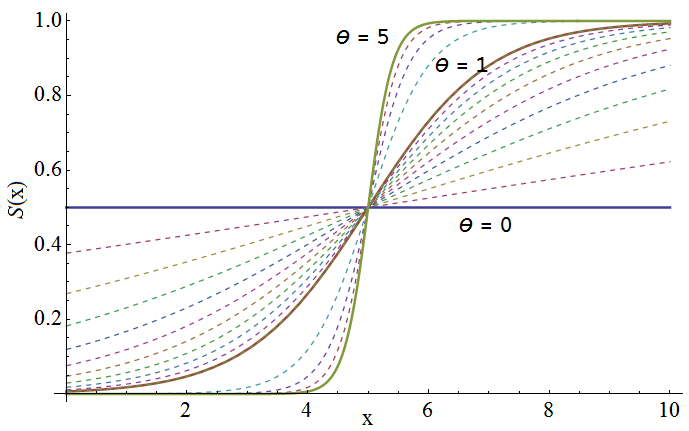
\includegraphics[width=\columnwidth]{../figures/sigmoid1.png}
\centering\caption{}\label{fig:sigmoid}
\end{figure}

\begin{figure*}[!ht]
\centering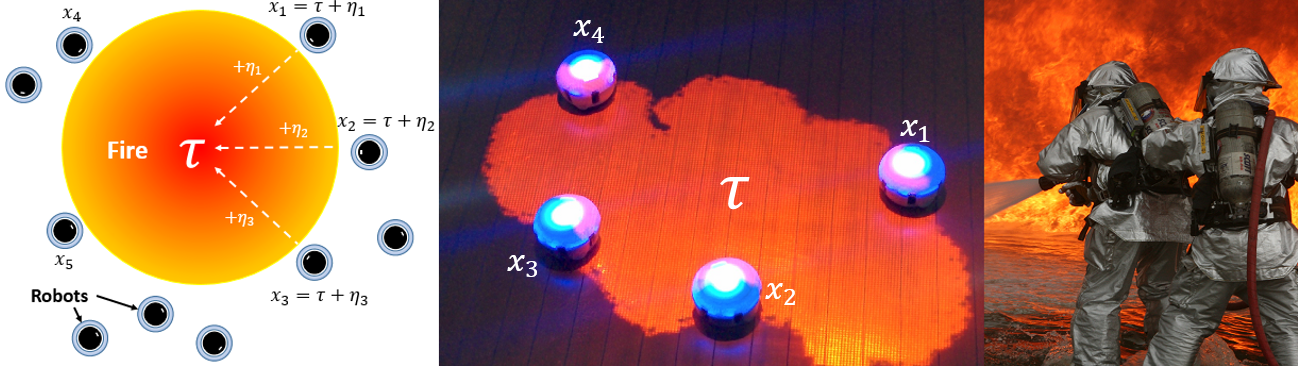
\includegraphics[width=\textwidth]{../figures/dropletfire.png}
\centering\caption{}\label{fig:dropletfire}
\end{figure*}

\section{Global Games: A Brief Overview}



\section{Collaboration Model}
We generalize a multi-agent collaboration scenario with the property of concurrent benefit as follows.

All tasks take place in a large operational area. Tasks or collaboration sites appear within the operational area at random but not necessarily uniformly spaced locations. All agents are dispersed uniformly and at random within the operational area. The reader should note that the act of searching for a collaboration site is arbitrarily chosen for the purposes of the model discussed in this paper; in practice, any search pattern or algorithm that best fits the scenario at hand may be chosen without affecting the conclusions provided by our model. Once an agent arrives at a collaboration site, it independently makes an estimate, $\tau$, for the group size required to successfully complete the task at that site. Agents at a task site employ a threshold based voting policy on whether or not to begin a collaborative action at that task site. The threshold function takes as input, that agent's estimate for the number of robots currently at the same collaboration site.

\begin{figure}
\centering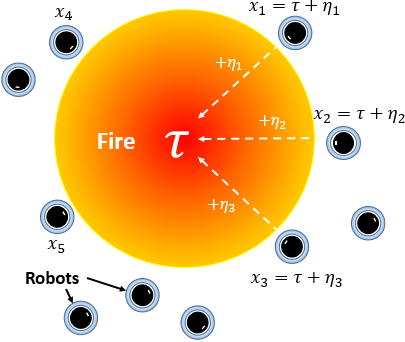
\includegraphics[width=\columnwidth]{../figures/globalgamesetup.png}
\centering\caption{}\label{fig:ggsetup}
\end{figure}

The signal received by an agent is,

\begin{equation}
	x_i = \theta + \eta_i
\end{equation}


\section{Results from Game Theory}
\subsection{Case I: Agents Not Sharing State Information}

\subsection{Case II: Agents Sharing State Information Perfectly}

\subsection{Case III: Agents Sharing State Information Imperfectly}

\subsection{Imperfect Knowledge of Group Size}




\section{Experimental Results}




\section{Discussion}




\section{Conclusion}



\section{Important Points}
- We define a class of tasks where there is a trade-off between time (waiting for more agents) vs probability of success (starting to work immediately).

- The Utility of the system is sigmoid in nature.

- Our approach accounts for errors in the model coming from robot sensors, inaccurate measurements, etc. (using variance in the sigmoid function)

- Introduce game theory language for a global game
  + Map the properties of a global game to the swarm system scenario being discussed

- Introduce mathematical terms that will be used in this paper

- Discuss all the assumptions being made about the swarm system

- Show that an equilibrium strategy for this global game without communication is to use a threshold function
  + Show that the sigmoid threshold function can be used to attain equilibrium
  + Support this result with real-robot experiments
  
- Discuss the impact of noisy communication of state information between agents  

%%%%%%%%%%%%%%%%%%%%%%%%%%%%%%%%%%%%%%%%%%%%%%%%%%%%%%%%%%%%%%%%%%%%%%%%%%%%%%%%
%%%%%%%%%   The Bibliography, if any   %%%%%%%%%
\bibliographystyle{plainnat}		% or "siam", or "alpha", etc.
%\nocite{*}						% list all refs in database, cited or not
\bibliography{../refworks}
\end{document}